% NeurReps / NeurIPS 2026 workshop format: 61 cm x 85 cm, portrait.
% Custom LaTeX poster; dimensions from official PosterInstructions (2026-11-02).
\documentclass{article}
\usepackage[paperwidth=61cm,paperheight=85cm,margin=0cm]{geometry}
\usepackage[T1]{fontenc}
\usepackage{lmodern}
\usepackage{amsmath,amssymb,graphicx,tikz,xcolor,qrcode}
\usepackage[hidelinks]{hyperref}
\renewcommand{\familydefault}{\sfdefault}
\pagestyle{empty}
\definecolor{ink}{HTML}{172D40}
\definecolor{teal}{HTML}{007D80}
\definecolor{pale}{HTML}{EAF5F3}
\definecolor{muted}{HTML}{4A5E69}
\definecolor{rulecolor}{HTML}{C7D8DB}
\newcommand{\bodyfont}{\fontsize{23}{30}\selectfont}
\newcommand{\smallfont}{\fontsize{21}{27}\selectfont}
\newcommand{\heading}[1]{{\color{teal}\fontsize{28}{33}\selectfont\bfseries #1}\par\vspace{.4cm}}
\newcommand{\place}[4]{\node[anchor=north west,inner sep=0pt,text width=#3cm,align=left] at (#1,-#2) {#4};}
\setlength{\parindent}{0pt}
\setlength{\parskip}{.35cm}
\hypersetup{pdftitle={Determinants of hyperparameter robustness in connectome reservoir computing},pdfauthor={Miles Walter Churchland and collaborators}}
\DeclareMathSizes{23}{23}{16}{12}
\DeclareMathSizes{21}{21}{15}{11}
\begin{document}
\null
\begin{tikzpicture}[remember picture,overlay,x=1cm,y=1cm]
\begin{scope}[shift={(current page.north west)}]
\fill[ink] (0,0) rectangle (61,-12.3);
\fill[teal] (0,-12.3) rectangle (61,-12.55);
\place{2}{1.25}{57}{{\color{white}\fontsize{17}{21}\selectfont\bfseries NeurReps 2026\hfill Symmetry and Geometry in Neural Representations}}
\place{2}{3}{57}{{\color{white}\fontsize{54}{62}\selectfont\bfseries Determinants of hyperparameter robustness\par in connectome reservoir computing}}
\place{2}{8.65}{57}{{\color{white}\fontsize{22}{28}\selectfont Miles Walter Churchland\textsuperscript{1}, Raul de Palma Aristides\textsuperscript{2}, Jordi Garcia-Ojalvo\textsuperscript{1},\par Anna Ritz\textsuperscript{3}, Greg Anderson\textsuperscript{4}, Miguel C. Soriano\textsuperscript{2}}}
\place{53.1}{4.0}{5.3}{{\color{white}\fontsize{15}{18}\selectfont\bfseries FULL PAPER}\par\vspace{.15cm}\href{https://arxiv.org/abs/2609.07355}{\begingroup\setlength{\fboxsep}{5mm}\colorbox{white}{\qrcode[height=3.4cm]{https://arxiv.org/abs/2609.07355}}\endgroup}\par\vspace{.1cm}{\color{white}\fontsize{13}{16}\selectfont arXiv:2609.07355}}
\place{2}{10.75}{57}{{\color{white}\fontsize{17}{21}\selectfont \textsuperscript{1}Universitat Pompeu Fabra\quad \textsuperscript{2}IFISC, CSIC--UIB\quad \textsuperscript{3}Biology, Reed College\quad \textsuperscript{4}Computer Science, Reed College}}


% Main finding: a full-width band, as in the layout sketch.
\fill[pale] (2,-13.4) rectangle (59,-17.5);
\place{2.8}{13.8}{55.4}{{\color{teal}\fontsize{16}{20}\selectfont\bfseries MAIN FINDING}\par\vspace{.1cm}{\color{ink}\fontsize{30}{36}\selectfont\bfseries Higher performance accompanies greater sensitivity to hyperparameter choice.}\par\vspace{.1cm}{\color{ink}\fontsize{20}{25}\selectfont The empirical \textit{C.~elegans} connectome occupies a relatively low-variance regime.}}

% Introduction and reservoir model.
\place{2}{18.6}{26.8}{\color{ink}\bodyfont
\heading{Research question}
\textbf{Which recurrent network features support robust computation?}
\par\vspace{.25cm}
Reservoir performance can vary substantially with hyperparameters. We compare a structured \textit{C.~elegans} connectome with controlled network variants to see which features support stable computation.
\par\vspace{.35cm}
\textbf{96 settings $\times$ 200 trials}\par
\smallfont Vary target spectral radius, leak rate, input scale, and bias. Robustness is the coefficient of variation (CV) across the 96 settings; \textbf{lower CV means greater robustness}.
\par\vspace{.35cm}
\textbf{IPC}: information processing capacity; nonlinear recall [2].\par
\textbf{KR}: kernel rank; history separation [3].\par
\textbf{MC}: memory capacity; recall of the past 30 inputs.
}
\place{31.5}{18.6}{27.5}{\color{ink}\bodyfont\heading{Reservoir computing}}
% The actual connectome is the fixed recurrent reservoir in this schematic.
\place{39.4}{21.2}{11.4}{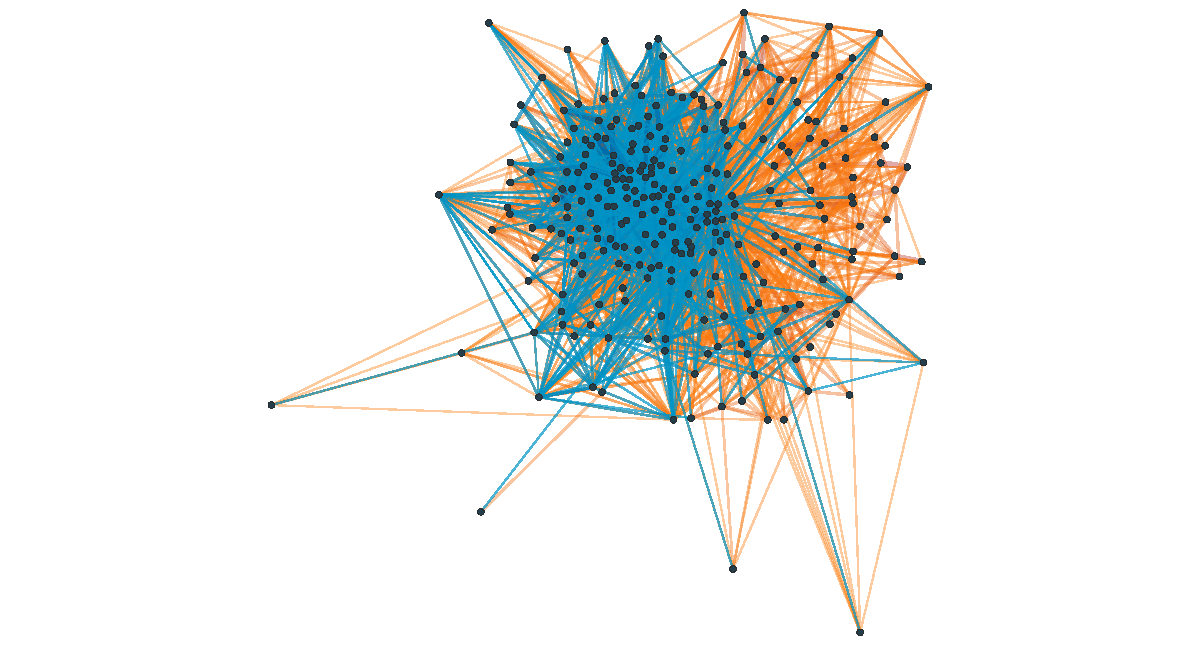
\includegraphics[trim=60 0 60 0,clip,width=11.4cm]{assets/connectome.pdf}}
\node[draw=teal,fill=pale,rounded corners=3pt,minimum width=4.6cm,minimum height=1.55cm,align=center,text=ink,font=\fontsize{18}{22}\selectfont] at (34.1,-25.0) {Scalar input\\$u_t$};
\node[draw=teal,fill=pale,rounded corners=3pt,minimum width=4.6cm,minimum height=1.55cm,align=center,text=ink,font=\fontsize{18}{22}\selectfont] at (55.9,-25.0) {Linear readout\\$y_t$};
% These fan-out / fan-in arrows are schematic, not a subset of actual inputs.
\foreach \y in {23.7,24.5,25.5,26.3} {
  \draw[-latex,muted,line width=1.15pt,opacity=.82] (36.55,-25) -- (43.0,-\y);
  \draw[-latex,muted,line width=1.15pt,opacity=.82] (49.0,-\y) -- (53.35,-25);
}
\place{38.1}{23.0}{3}{{\color{muted}\fontsize{17}{21}\selectfont $W^{\mathrm{in}}$}}
\place{50.4}{23.0}{3}{{\color{muted}\fontsize{17}{21}\selectfont $W^{\mathrm{out}}$}}
\place{40.9}{29.05}{9}{{\color{teal}\fontsize{17}{21}\selectfont\bfseries Fixed reservoir}}
\place{54}{26.1}{5}{{\color{muted}\fontsize{16}{19}\selectfont Trained}}
\place{31.5}{30.6}{27.5}{\color{ink}\smallfont
Input reaches \textbf{all 297 neurons} via Gaussian weights of either sign, fixed per trial up to input scaling; the trained readout combines their states. Gray arrows show direction, not sign. \textit{C.~elegans} connectome: 3,604 chemical edges [1]; largest component shown. Recurrent edges: {\color{orange!80!black}positive}; {\color{blue!65!cyan}negative.} Edge directions omitted.
}
% Light rules separate the four regions without competing with the figures.
\draw[rulecolor,line width=1pt] (30,-18.8) -- (30,-34.4);
\draw[rulecolor,line width=1pt] (2,-34.8) -- (59,-34.8);
\draw[rulecolor,line width=1pt] (30,-35.6) -- (30,-75.9);

% Results: left and right panels, following the reference sketch.
\place{2}{35.6}{27.5}{\color{ink}\bodyfont
\heading{Architecture tradeoff}
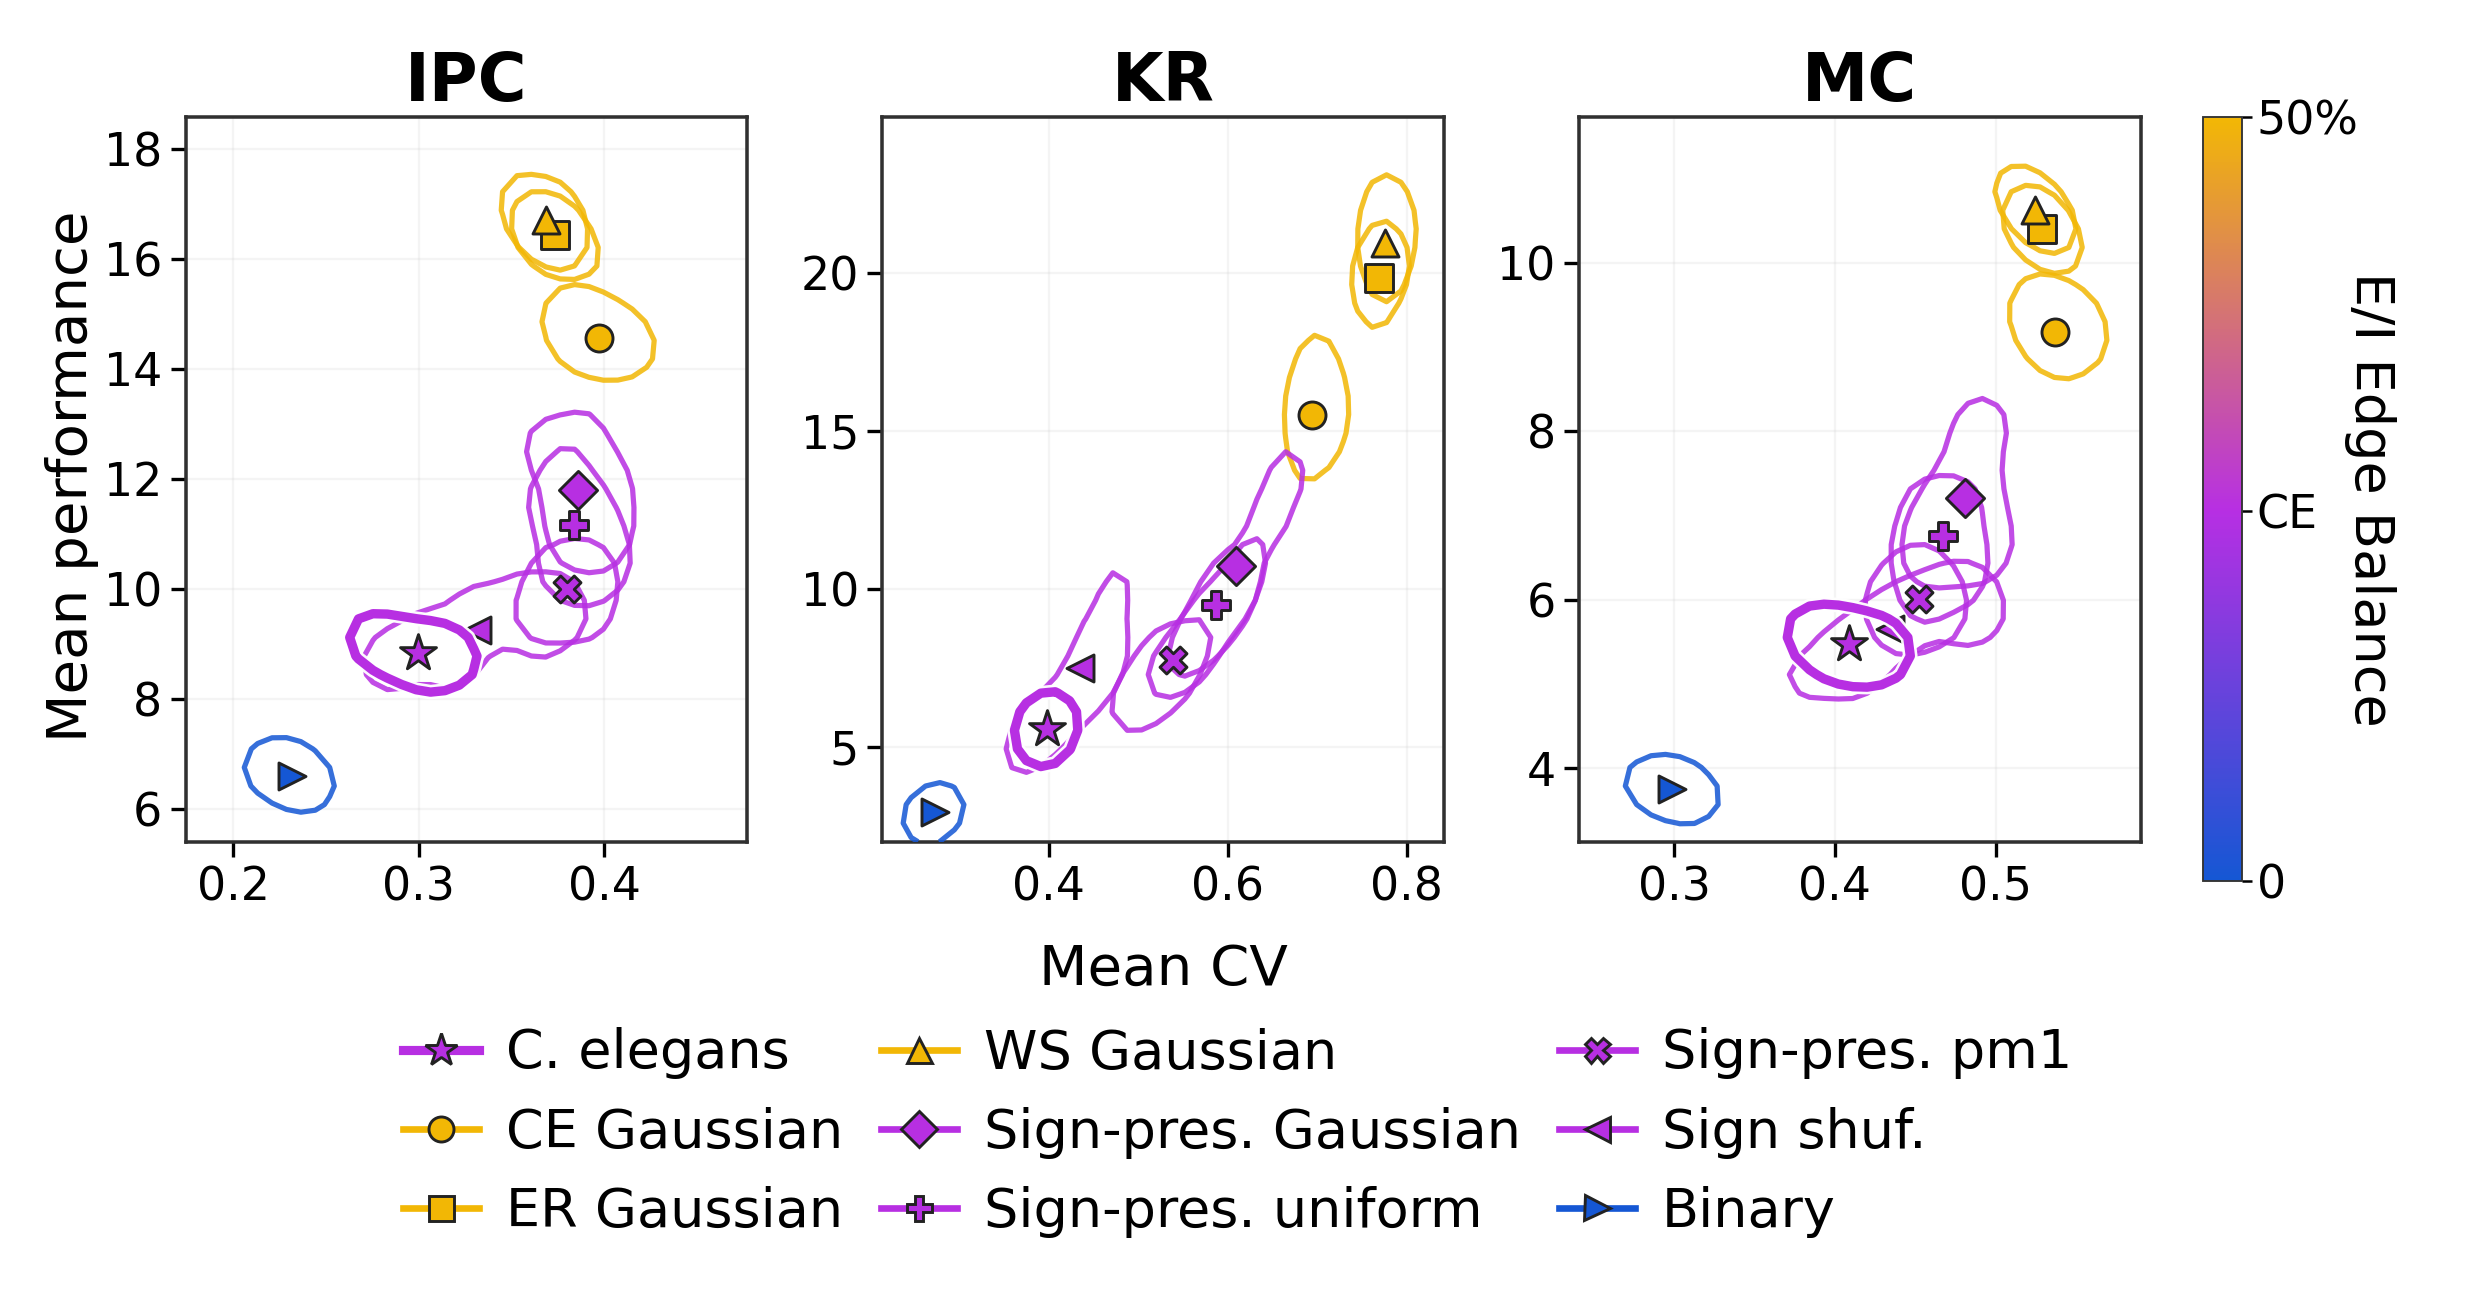
\includegraphics[width=27.5cm]{assets/architecture_tradeoff.png}
\par\vspace{.2cm}\smallfont
\textbf{Higher performance accompanies higher CV.} Mean performance is averaged across 96 settings. Contours enclose the highest-density 50\% of trials; markers identify architectures.
\par
Colors show excitatory/inhibitory (E/I) edge balance: 0\%, CE $\approx24.25\%$, and 50\%. CE: \textit{C.~elegans}; ER: Erd\H{o}s--R\'enyi; WS: Watts--Strogatz. Sign-pres.: signs preserved; sign shuf.: signs shuffled; pm1: $\pm1$ weights.
\par\vspace{.35cm}\bodyfont
\textbf{Takeaway.} The empirical connectome lies on the lower-sensitivity side of the performance--robustness tradeoff.
}
\place{31.5}{35.6}{27.5}{\color{ink}\bodyfont
\heading{E/I edge balance}
\makebox[27.5cm][c]{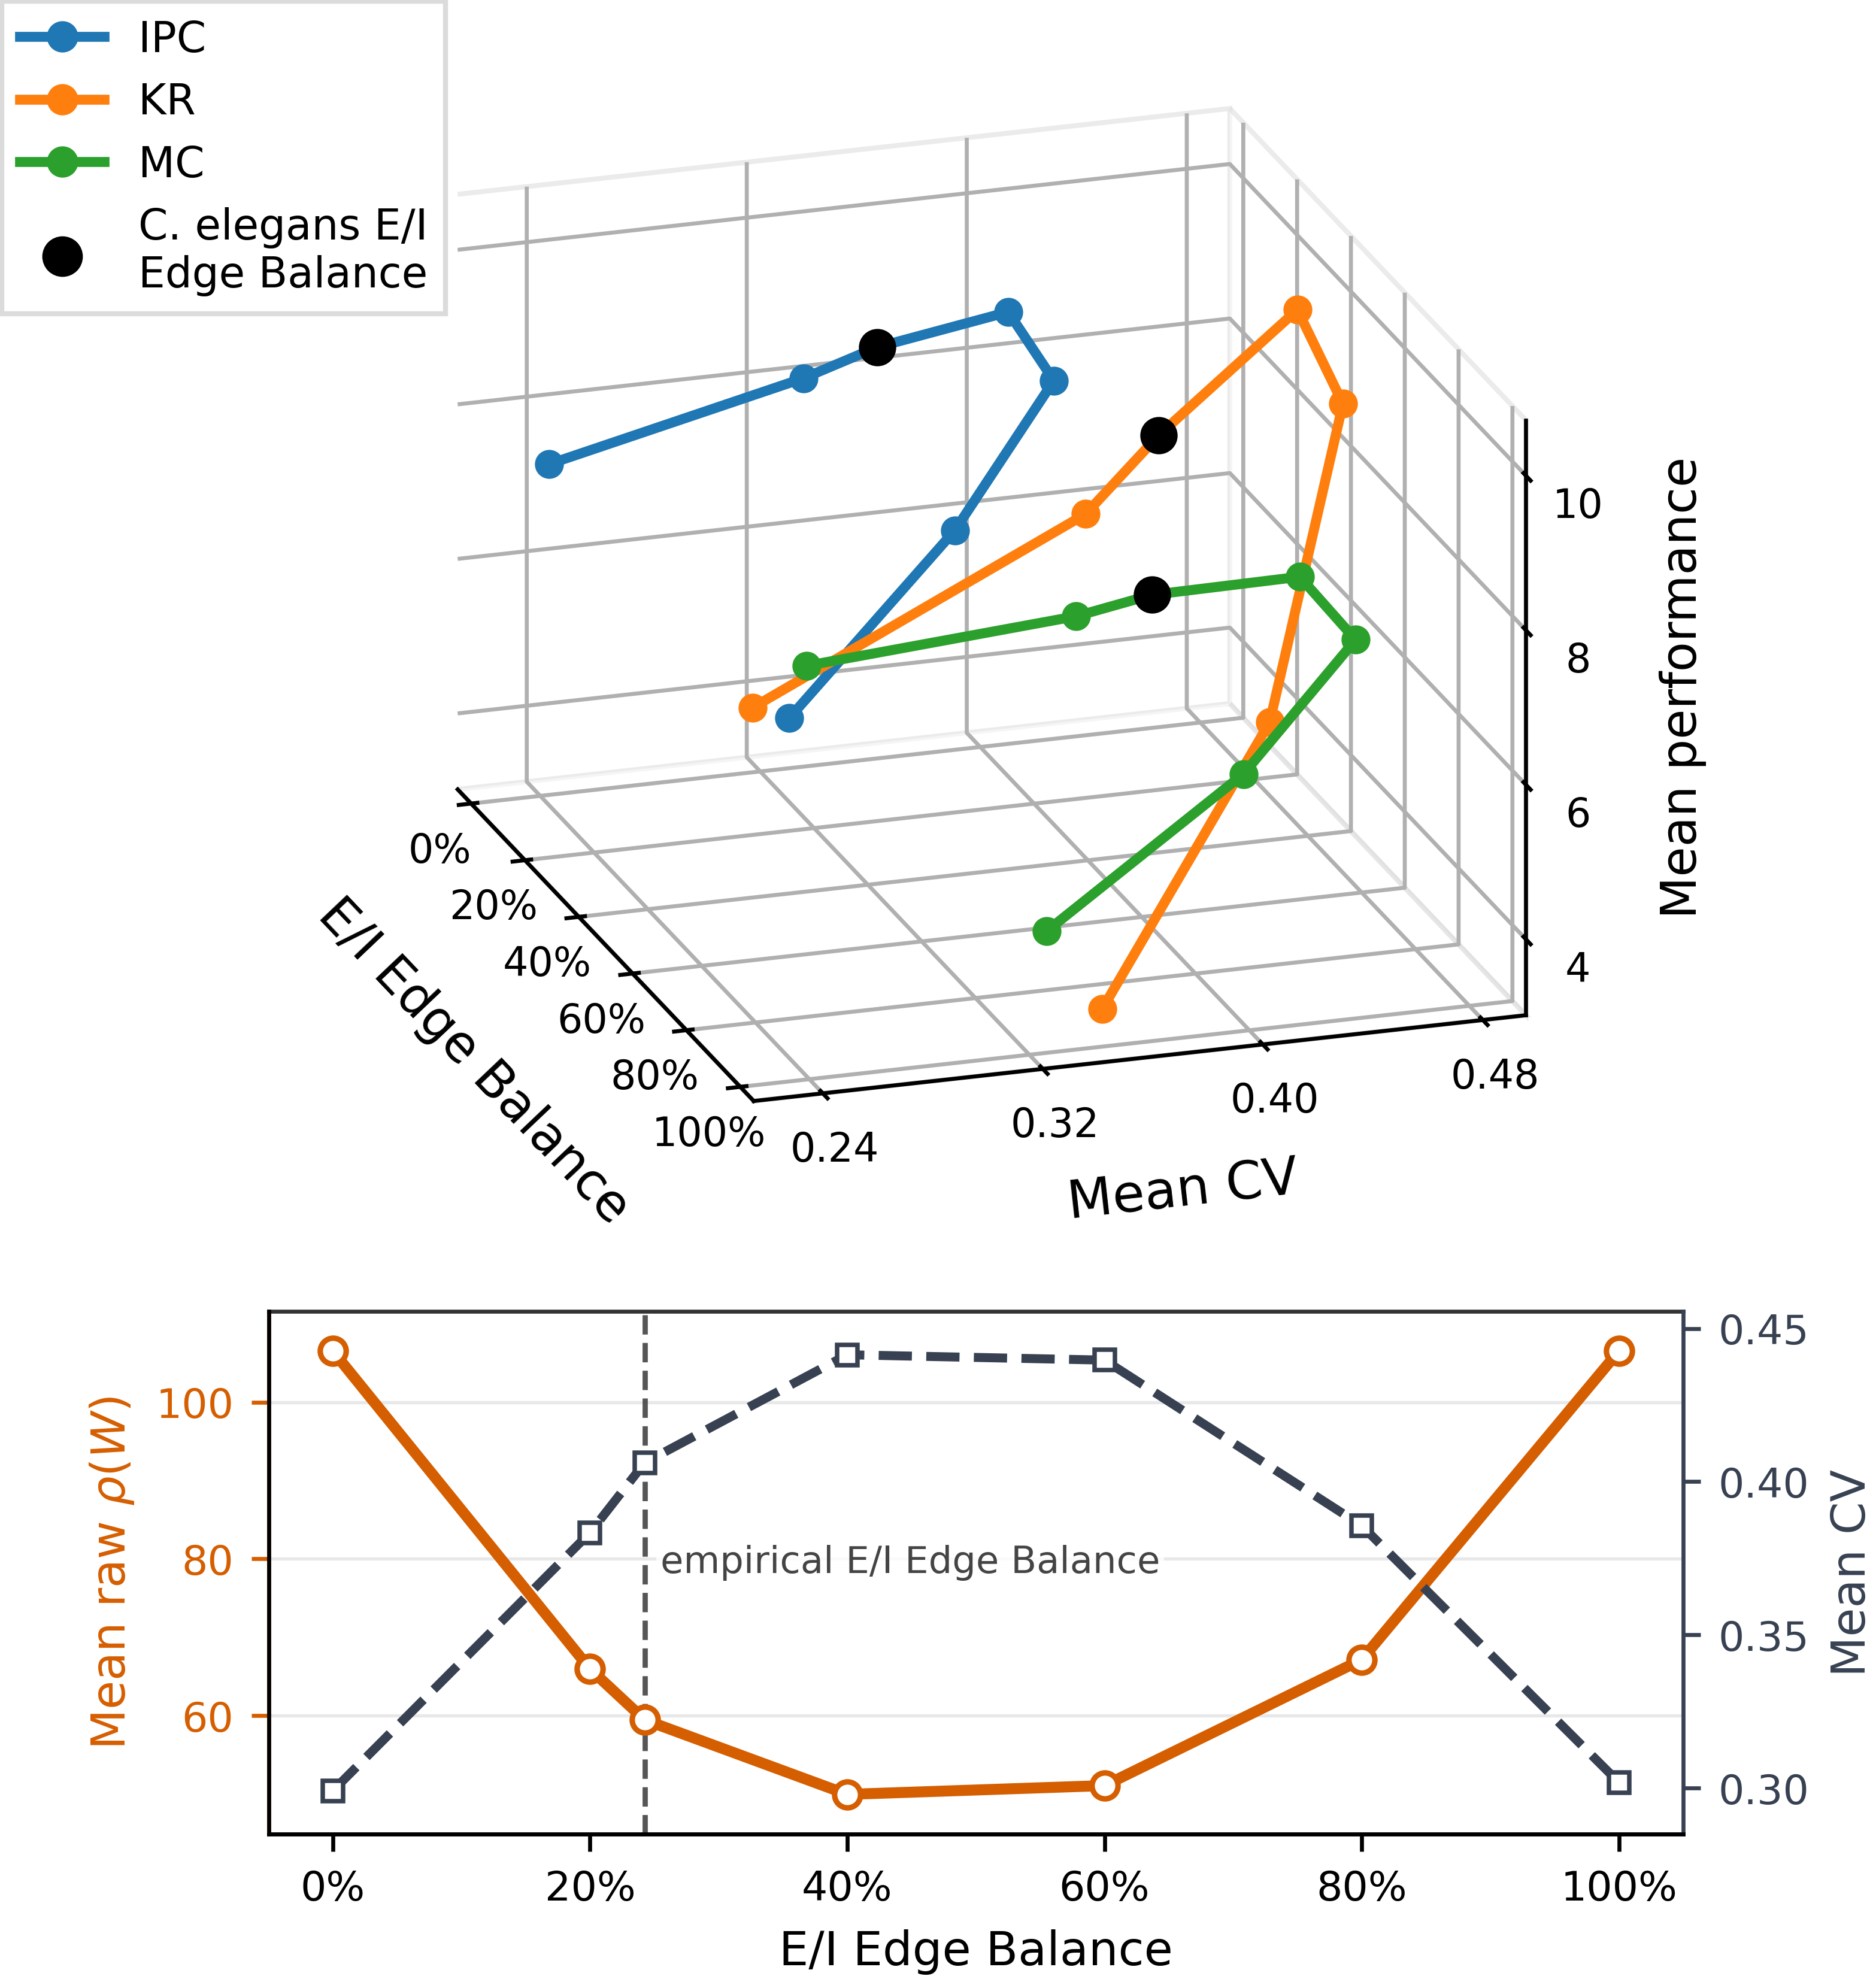
\includegraphics[width=23.5cm]{assets/performance_robustness_curves.png}}
\par\vspace{.15cm}\smallfont
\textbf{Changing E/I edge balance moves performance and CV together.} Top: IPC, KR and MC; black markers indicate the empirical balance. Bottom: raw spectral radius and CV averaged across metrics. Points average 200 trials.
\par\vspace{.2cm}
\textbf{Normalization matters.} At the same target radius, lower raw radius requires a larger recurrent-weight scaling factor. The observed tradeoff combines sign-structure changes and normalization-induced rescaling; these effects are not isolated.
}
\fill[pale] (2,-64.5) rectangle (29.5,-70.0);
\place{2.8}{65.0}{25.9}{{\color{teal}\fontsize{22}{27}\selectfont\bfseries How to read the tradeoff}\par\vspace{.2cm}{\color{ink}\fontsize{21}{27}\selectfont In the architecture plots, moving up means higher performance; moving right means greater sensitivity to hyperparameter settings. The empirical connectome lies toward the lower-left.}}
\fill[pale] (2,-76.7) rectangle (59,-80.1);
\place{2.7}{77.15}{55.6}{\color{ink}\smallfont\textbf{Scope and limitations.} Robustness here means low relative variation across the tested hyperparameter grid; it does not imply invariance to all parameter changes. IPC omits products across different delays. Of 3,604 chemical edges, 1,864 have unknown or complex signs and are assigned signs to match the labeled-edge ratio; selected controls remove them. Electrical synapses and self-loops are excluded; input reaches all units.}
\place{2}{81}{57}{\color{muted}\fontsize{13}{17}\selectfont
\textbf{Selected references}\quad
[1] Fenyves et al. (2020). Synaptic polarity and sign-balance prediction. \textit{PLOS Comput. Biol.} 16, e1007974.\par
[2] Dambre et al. (2012). Information processing capacity of dynamical systems. \textit{Sci. Rep.} 2, 514.\par
[3] Roy \& Vetterli (2007). The effective rank: a measure of effective dimensionality. \textit{EUSIPCO}, 606--610.}
\end{scope}
\end{tikzpicture}
\end{document}
